
\subsection{Experiment Design}
\label{sec:methtrain}
Previously, we described the ideal model of our measurement method,
which explained the idea and workflow at a high-level. However, this model
does not take into consideration packet loss or extra traffic at the
{\reflector}. As one would expect, these assumptions are unrealistic in a real
world scenario, as packet loss can happen at many stages along the path.
Furthermore, there is no guarantee that the host with an open port online
will not receive any other traffic. Thus, to perform the measurement in the real
world, we need to take all these factors into consideration and make sure
that our analysis model is robust to these real world uncertainties.

Moreover, our detection methodology also needs to be \textit{efficient},
\textit{accurate}, and have \textit{low overhead}. Since we need to
measure every pair of \texttt{({\reflector}, IP)}, which is a
very large number, and the blacklist content changes rapidly, the detection
method needs to be efficient so that we can finish the measurement in a
reasonable amount of time. The method should also have a low false positive
and false negative rate, so we can be confident about the result. Finally, it
should require as few packets as possible, both to meet network bandwidth
limitations on our measurement machine side and reduce impact on
{\reflectors}.

We define a \textit{trial} as a single measurement that tests if a
{\reflector} blocks a blacklist IP. Figure~\ref{fig:design_implementation}
shows the process of one trial in detail. For each trial, the measurement
machine sends five consecutive \textit{probe packets} to the {\reflector},
with each packet being sent one second apart. In our experiment, the probe
packets are TCP SYN-ACK packets and we get IP IDs from response RST packets.
Between the third and fourth probe packets, the measurement machine sends
five \textit{spoofed packets}, also TCP SYN-ACK, with source IPs equal to the
blacklist IP. And between the fourth and the fifth probe packets, it sends
another five spoofed packets. Each time we send the five spoofed packets, we
send them 0.15 second apart consecutively, spreading them across the one-second
window between two IP ID probes.

\begin{figure}[t]
\centering
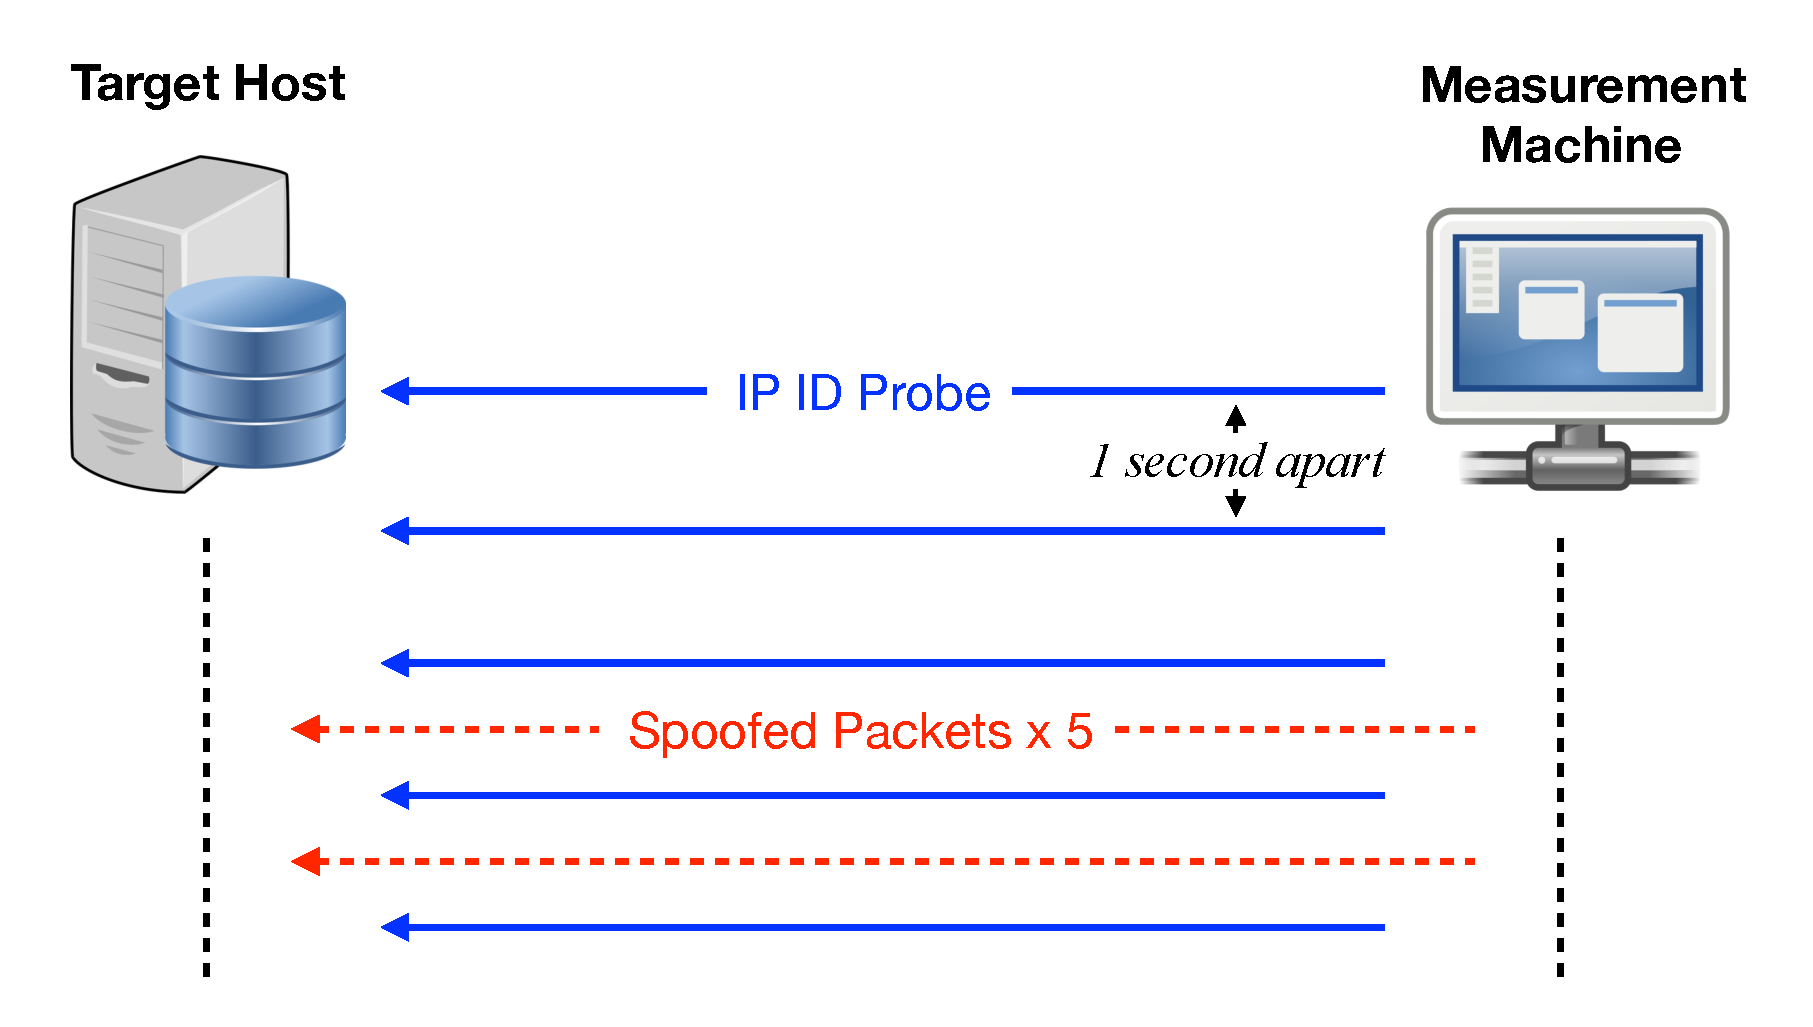
\includegraphics[width=0.85\columnwidth]{images/croped_design_implementation.pdf}
\caption{Blocking detection methodology. The solid blue lines are the \textit{probe
packets}. Dashed red lines are the \textit{spoofed packets}. The spoofed
packets impersonating blacklist IPs trigger the increase of the
{\reflectors}' IP ID. The IP ID of responses to probe packets are used to
determine blocking behavior.}
\label{fig:design_implementation}
\end{figure}

Now, we inspect the increases between the IP IDs for the packets received by the
measurement machine. In an ideal world, when there is no other traffic
generated by the {\reflector}, and no packet loss during our measurement, we
should observe that the IP ID increases between consecutive probes by exactly
1, and for the last two deltas, since we send the spoofed packets in between
our probe packets, the final IP ID increases will be different based on the
host's blocking behavior.

If the {\reflector} does not block the blacklist IP, then
we will observe an IP ID increase sequence in our received RST responses as:
\[[\hspace{0.1cm} +1, +1, +6, +6 \hspace{0.1cm}]\]
Here the last two deltas are +6 since the {\reflector} does not block the
blacklist IP and thus responds to spoofed packets, causing IP ID to increase by
5, and our probe packet causes it to increase by another 1, which together make +6.

On the other hand, if the {\reflector} blocks the blacklist IP, then we will see an IP
ID increase sequence as:
\[ [\hspace{0.1cm} +1, +1, +1, +1 \hspace{0.1cm}] \]
Here the last two deltas are +1 since the {\reflector} blocks the blacklist IP,
leading to no extra change in IP ID.
%\textcolor{red}{maybe have an example of what happens when we do not see ideal conditions}

The first three probes --- corresponding to the first two IP ID deltas --- act as a
control. The last two ``probe and spoof'' patterns perform the actual measurement.
Seeing the initial two ``+1'' indicates this host is in a quiet period --- no
extra network traffic. Therefore, we can be more confident that the following
IP ID jump (``+6'' in our case) is because of our experiment. However,
while we present the choice of the numbers in the experiment as fait accompli,
there is a rationale behind the choice of numbers which we discuss in Section~\ref{subsec:fpfn_analysis}.

\subsubsection{Inference Criteria}
%\textbf{Inference Criteria: }
Now we discuss how to infer whether a {\reflector} is blocking a blacklist IP
in the real world. We have limited vantage points from the measurement machine, as
such, and our information is limited to the IP IDs we see from the {\reflector}.
Therefore, we would like to be very conservative when making a judgment. In this
measurement, our approach is to try the same trial, between a {\reflector} and a
blacklist IP, many times until we get a ``perfect signal'' --- a response
which matches all the criteria below:

\begin{enumerate}
    \item The measurement machine received exactly five RST responses from the {\reflector}.
    \item The five responses are received one second apart consecutively.
    \item The IP ID increase sequence in the five responses are either [+1, +1, +6, +6],
    which we will conclude as no blocking, or [+1, +1, +1, +1], which we will
    conclude as blocking.
    \item If any of the above three criteria are not met, we repeat the same experiment
    again. We repeat up to 15 times before giving up.
\end{enumerate}

Essentially, the first requirement ensures no packet loss. The second
requirement ensures responses we received reflect the real IP ID changes in
the {\reflector}. The Internet does not guarantee the order of packet arrival.
Although we send one probe packet per second, and send the spoofed
packets in between of the probe packets, these packets might not arrive at
the {\reflector} in the same order. There is a similar case for response packets.
Therefore, the IP ID sequence we get from the response packets
might not represent the real order of IP ID changes in the host. Requiring
that
the received response packets are also close to 1 second apart, we minimize
the probability of the reordered packets. In our experiment, we enforce that
the response packets can not be less than 0.85 or more than 1.15 seconds
apart.

The third requirement is the core of our inference logic. We want to be
conservative when concluding whether there is blocking or not, so we will
make the judgment only when we observe an IP ID increase sequence [+1, +1, +1,
+1] or [+1, +1, +6, +6], and ignore everything else. Then if we saw a
sequence of [+1, +1, +1, +1] but the host is not blocking the blacklist IP,
that would mean all the 10 spoofed packets were lost during the transmit. On
the other hand, if we see [+1, +1, +6, +6] and the host is actually blocking
the blacklist IP, then that would mean during our experiment, there are
exactly five extra packets generated by the host during each of the last two
windows. Both cases are very unlikely to happen, and we will show a concrete
analysis of false positives and false negatives in the remainder of this section.


\subsubsection{False Positive and False Negative Analysis}
\label{subsec:fpfn_analysis}
%\textbf{False Positive and False Negative Analysis: }
For our experiment, a ``false positive'' is when a host is not
blocking a blacklist IP, but we mistakenly conclude it is blocking. On the
other hand, a ``false negative'' is when a host is blocking a
blacklist IP, but we mistakenly conclude it is not blocking. With
{\reflectors} being collected, we can empirically evaluate the
probability of a false positive or a false negative precisely.

For false positive evaluation, we first acquire a list of IPs that are verifiably
not being blocked by {\reflectors}. Since we own these IPs, we can easily verify
that by directly probing {\reflectors} from these IPs. We acquired and tested
1,265 IPs from five different /24s. Then we probe {\reflectors} and send the
spoofed packets with source addresses set to these pre-selected IPs. Since we
know that these IPs are not blocked, if we observe an IP ID increase sequence of
[+1, +1, +1, +1], then we know it is a false positive.

For false negative, we run the experiment with only probe packets, and no
spoofed packets. This is equivalent to the scenario where the host blocks the
spoofed IP. Then if we observe an IP ID increase sequence of [+1, +1, +6,
+6], then we know it was due to the background traffic at the {\reflector}
and hence is a false negative.

Although we have presented the design where we spoof five packets
in each of the last two seconds, we also experimented with a range of
numbers and calculated their false positive and negative rates. We tested
with spoofed packets equal to 3, 4, 5, 6, 7 respectively. For each number,
we use 15 distinct IPs we own as the source addresses to spoof, and we
create another group with 15 place holder IPs where we do not send spoofed
packets during the experiment. We run each experiment twice, and the final
results are shown in Figure~\ref{fig:fp_fn_analysis}.

%Our goal is to minimize the false positives and false negatives while also keeping
%in mind the amount of traffic we generate. Additionally, we have a few dimensions
%of the experiment which we can adjust to reach this goal. Namely, the number of
%packets we spoof, and the number of times we spoof.
%To find these optimal numbers, we test with a range of numbers and calculate

\begin{figure}[t]
\centering
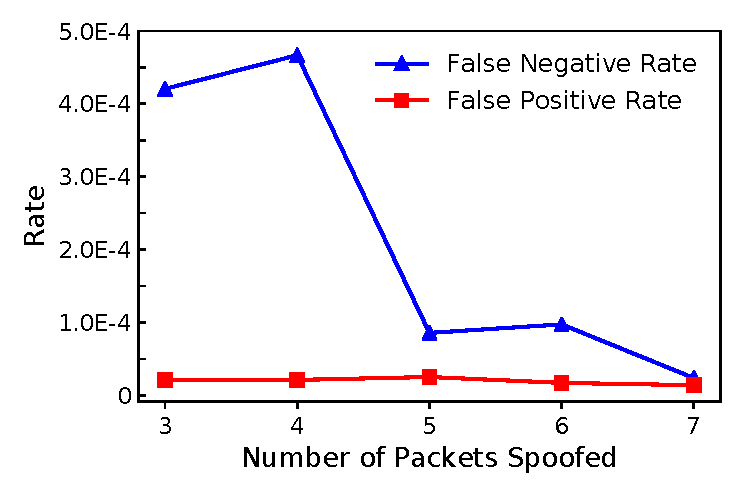
\includegraphics[width=0.85\columnwidth]{images/false_positive_negative.pdf}
\caption{False positive rates and false negative rates of the technique when
spoofing different amount of packets. We choose number 5 as a trade-off
between low false positive and negative rates, and as few packets being sent
to reflectors as possible.}
\label{fig:fp_fn_analysis}
\end{figure}

A few things stand out. The false negative rate drops significantly when we
send 5 spoofed packets. Surprisingly, the false negative rate jumps up
slightly when we spoof 6 packets. On the other hand, the false positive rate
keeps marginally trending downwards as we increase the number of spoofed
packets. We try to make the trade-off between having low false positive and
negative rates, but at the same time generating as little traffic as possible.
We choose 5 spoofed packets as a balance. By sending 5 spoofed packets, we
get a false positive rate of 2.5e-5, and a false negative rate of 8.5e-5.

Furthermore, we also experimented with strategies where we send 4 probe packets, from which
we get 3 IP ID deltas, and sending 6 probe packets, from which we get 5 IP ID
deltas. With only 3 deltas we suffer a higher false negative rate, as it is
easier for the {\reflector} to show the same IP ID increase sequence with
extra traffic. With 6 probes, on the other hand, we prolong the experiment,
and more importantly, it is harder for us to get the ``perfect signal'' since
it is harder to capture a period with no other traffic when the time window
is longer. Thus, our choice of 5 probe packets with 5 spoofed packets in
between is a trade-off between multiple factors.

%We choose to send 5 probe packets because it is a balance between getting
%enough sample point of IP ID to see the changes, and not sending too many
%packets to the {\reflector} that might affect the host, as we need to repeat
%the experiment many times for many different blacklist IPs. The first three
%probes (where we get the first two IP ID delta) act as a control, and the
%last two probe and the spoof packets serve the actually experiment. The
%choice of 5 spoofed packets between each second is also the result of
%balance. If we send too little spoofed packets, then it is hard to argue
%whether the additional IP ID increments come from our spoofed packets or the
%hosts' own third-party traffic. If we send too many spoofed packets, it is
%hard to ensure they will arrive the host exactly between the probe packets,
%and also might trigger some stateful firewall logic, as we discussed in
%Section~\ref{sec:requirement}.

\subsection{Control Group}
\label{sec:methvalid}
%\noteby{KL}{Here we
%    should describe additional validation, such as testing whether popular sites
%    are being blocked, and any other validation steps, such as repeating the
%    measurement, that we do. The part where we confirm our findings by asking
%    universities about their blocking policy can remain in the analysis section.}
To further validate our measurements, every time we test a set of
blacklist IPs against each reflector, we also include a control group
of 20 randomly chosen IPs. These IPs are chosen from networks
geo-located in the United States. We further ensure they do not
appear on any of our blacklists, they are BGP routable, and they are
not from the same ASes as the {\reflectors}. The purpose of the
control group is to create a random set of IPs that are unlikely to be
blocked in bulk by a {\reflector}. We use US IPs to avoid the
potential problem of geo-blocking. If a {\reflector} does block a
significant fraction of control IPs, it is probably because the
{\reflector} is not suitable for this methodology (one reason can be
that our ingress-filtering step did not catch these IPs). We discover
91 reflectors that constantly show blocking behavior for all control
IPs, while the remaining reflectors never block more than 10 of the
control IPs. We conclude that these 91 reflectors are not useful for
measurement, and remove them from our total reflector set.

\subsection{Ethical Considerations}
\label{sec:ethics}

In general, we do not think our measurement will cause any harm to the
reflectors. But to be further cautious, we take effort to minimize the
measurement packets we send to each reflector, as described in
Section~\ref{sec:methtrain}. Moreover, we will not disclose the exact
identity of any reflector in this paper, and only report aggregated
numbers.

%\subsection{Tor Blacklist Placeholder}
%Note that the {\ettor} includes IPs from all nodes involved in Tor
%networks, including entry nodes, so the {\reflectors} who block this
%list cannot use Tor services themselves.  As a result, this Tor list
%is more broad than Tor exit blocking, in which a host only blocks exit
%nodes so other hosts cannot access their service from Tor (but the
%blocking host can still access the Tor network itself).
%\noteby{GV}{Why define the Tor blacklist here?  Perhaps move to
%  blacklist selection or validation?}
